\section{Modes of Parallel Execution}

Parallelism in test execution can be achieved at different levels.
Figure~\ref{fig:levels} illustrates that.\Fix{...}  This paper focuses
at lower-level parallelism that can be achieved through build systems
and testing frameworks.  In the following we elaborate relevant
features of these components focusing on Java, Maven, and JUnit but
the discussion can be generalized to other languages, build systems,
and testing frameworks.

\subsection{Build Systems}
Build systems, such as Maven\footnote{\url{maven.apache.org}},
typically provide the option to \emph{fork} JVM instances
proportionally to available cores in the machine.  If the option
``fork JVM'' is enabled, Maven will allocate a user-provided number of
JVM instances to each core in the machine and will allocate each test
class to exactly one JVM.  Note that there is no guarantee to
uniformly distribute load to each JVM given that the build system uses
classes as the unit to specify test tasks.\Fix{we need to know how
  Maven allocates test classes to JVMs}

\subsection{Testing Framework}

The list below shortly describes the choices to control parallelism
within each JVM.

\begin{figure}[t!]
  \centering
  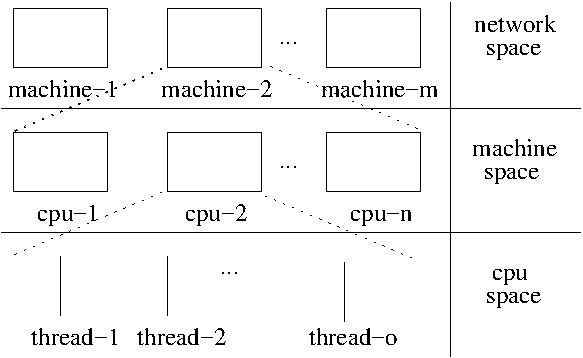
\includegraphics[width=0.4\textwidth]{figs/parallel-levels.pdf}
  \caption{\label{fig:levels}Levels of parallelism.}
\end{figure}

\newcommand{\Seq}{L0}
\newcommand{\ParClassSeqMeth}{L1}
\newcommand{\SeqClassParMeth}{L2}
\newcommand{\ParClassParMeth}{L3}

\begin{itemize}
\item \textbf{Sequential (\Seq).}~This configuration results in
  sequential execution of test classes and their methods, according to
  the order defined in the testing framework\Fix{cite}.  For JUnit
  this is the default configuration.
\item \textbf{Sequential classes; parallel methods
  (\ParClassSeqMeth{}).} This configuration results in the sequential
  execution of the test classes assigned to the JVM.  However, within
  each class, test methods run in parallel.\Fix{are there options to
    limit number of threads or a thread per test method?  Do they use
    thread pools?  etc....}
\item \textbf{Parallel classes; sequential methods
  (\SeqClassParMeth{}).}  This configuration results in the parallel
  execution of test classes but test methods of any given class are
  executed sequentially.\Fix{one thread per class?  if not, what
    classes are scheduled to execute first?}
\item \textbf{Parallel methods (\ParClassParMeth).} This configuration
  results in parallel execution of any given test method of any class.
\end{itemize}

\Fix{We need a par. providing rationale in to explain (points in favor/against) these choices.}
